\documentclass[aps,prd,10pt,twocolumn,nofootinbib,superscriptaddress]{revtex4-2}
\usepackage{amsmath,amssymb}
\usepackage{graphicx}
\usepackage{url}
\usepackage{hyperref}

% Near-final manuscript for expert feedback before journal submission.
\begin{document}

\title{A Ringdown-Readiness Framework for Beyond-Kerr Claims: Public GW250114 Projections and Static QNM Benchmarks}
\author{J. Vrba}
\affiliation{Research Centre for Theoretical Physics and Astrophysics, Institute of Physics, Silesian University in Opava, Bezru\v{c}ovo n\'am.~13, 746\,01, Opava, CZ}


\begin{abstract}

In the present work we formulate a reproducible ringdown-readiness framework
for beyond-Kerr claims. The motivation is simple: a phenomenological black-hole
metric is not ready for gravitational-ringdown use only because it has a
horizon, photon ring, ISCO, QPO fit, or shadow. A ringdown test also requires
the perturbation problem, boundary conditions, and reproducible quasinormal
mode spectra. We illustrate the framework in two complementary ways. First, we
use public GW250114 spectroscopy products and published higher-derivative Kerr
QNM fingerprints to make a transparent public-data projection. In this worked
example the Kerr value $\alpha=0$ remains inside every one-at-a-time 90
percent interval, with the largest nominal displacement equal to $0.497\sigma$
for the RINGDOWN branch and $1.222\sigma$ for the pyRing branch. The two public
branches are mutually consistent, with maximum normalized projection
difference $0.535\sigma$. This null result is not advertised as an evidence
ratio or as a full beyond-Kerr reanalysis; it is a reproducible benchmark for
what can be inferred from public ringdown products alone. Second, we validate
$25$ static supplied-potential rows for Schwarzschild, braneworld tidal charge,
Bardeen, and Hayward examples as static QNM benchmarks. These static benchmarks
are not GW250114 constraints on rotating remnants. They demonstrate, however,
where metric-only phenomenology ends and where gravitational-ringdown readiness
begins.

\end{abstract}
\maketitle
\section{Introduction}

Black-hole ringdown spectroscopy is becoming an important test of the Kerr
description of compact-object remnants \cite{Ber-Car-Sta:2009:CQG:,Isi-Gie-Far:2019:PRL:,Gho-Bri-Buo:2021:PRD:}.
In general relativity, the late post-merger signal is described by a discrete
set of quasinormal modes. Their frequencies and damping times are fixed by the
remnant mass and spin. When the signal-to-noise ratio is high enough, measured
ringdown quantities can therefore be compared with the Kerr pattern and used
as a test of the strong-field regime.

This program is powerful, but it also imposes a strict theoretical standard.
A metric alone is not a gravitational ringdown model. A line element may be
useful for geodesic phenomenology, QPO modelling, ray tracing, or shadow
studies \cite{Joh:2013:PRD:,Kon-Rez-Zhi:2016:PRD:,Ped-Vag:2024:PRD:},
but gravitational ringdown additionally requires a perturbation problem, the
relevant propagating degrees of freedom, boundary conditions, and reproducible
QNM spectra. Without these ingredients it is not clear what quantity should be
compared with the observed ringdown frequencies and damping times.

The aim of this paper is to make this distinction operational. We propose a
ringdown-readiness framework for beyond-Kerr claims and illustrate it with two
controlled examples. The first example is observationally motivated: we use
public GW250114 RINGDOWN and pyRing products
\cite{LIG-Vir-KAG:2025:ARXIV:,LIG-Vir-KAG:2025:ZENODO:} to project published
higher-derivative Kerr QNM fingerprints \cite{Can-Cap-Fra:2024:ARXIV:,Can-Fra-Her:2023:ARXIV:,Can-etal:2024:GITHUB:}
onto one-at-a-time effective couplings. This is not a full strain-level
beyond-Kerr inference. It is a reproducible public-data projection showing how
theory-backed rotating QNM fingerprints can be confronted with public
spectroscopy products.

The second example is theory-readiness motivated. We validate supplied
gravitational master-potential examples for static spherical backgrounds,
including Schwarzschild, braneworld tidal charge, Bardeen, and Hayward cases
\cite{Ber-Car-Sta:2009:CQG:,Tos-Stu-Sch:2016:PRD:,Ulh:2014:BJP:,Bol-Skv:2025:ARXIV:}.
This part is not a direct constraint on the GW250114 remnant, which is a
rotating object. Its role is different: it demonstrates a reproducible
benchmark level between metric-only phenomenology and a theory-backed
rotating-ringdown calculation.

The central message is therefore methodological. Public GW250114 products can
be used for transparent sanity checks when a model supplies rotating QNM
fingerprints. Static supplied-potential benchmarks can be used to test whether
phenomenological metrics have reached at least a reproducible perturbative
level. Metric-only models remain below the threshold required for
observational gravitational-ringdown claims.

This framing is meant to be useful in practice. It does not forbid the use of
phenomenological metrics in QPO, shadow, plasma, or geodesic calculations. It
only says that, when the same metric is promoted to a ringdown statement, the
paper must also supply the perturbation system or an equivalent validated QNM
fingerprint. The readiness ladder is therefore a referee-facing diagnostic:
it tells the reader what has actually been tested and what has merely been
assumed.

\section{Methods}

\subsection{Readiness Logic}

We use the term ringdown-ready in a narrow sense. A model is not ringdown-ready
only because it specifies a metric. It must also specify enough perturbation
physics to compute gravitational QNM spectra. In the present paper we use the
following ladder:

\begin{itemize}
\item metric/geodesic only;
\item test-field QNM;
\item supplied gravitational master potential;
\item validated static gravitational QNM;
\item theory-backed rotating gravitational QNM.
\end{itemize}

The public GW250114 projection uses the highest level available in this work:
published rotating Kerr-like QNM fingerprints for higher-derivative
corrections. The static branch reaches the validated static gravitational-QNM
level for selected examples. It does not claim to replace a theory-backed
rotating calculation.

\begin{figure*}[t]
\centering
\IfFileExists{figures/static_metric_readiness_ladder.pdf}{%
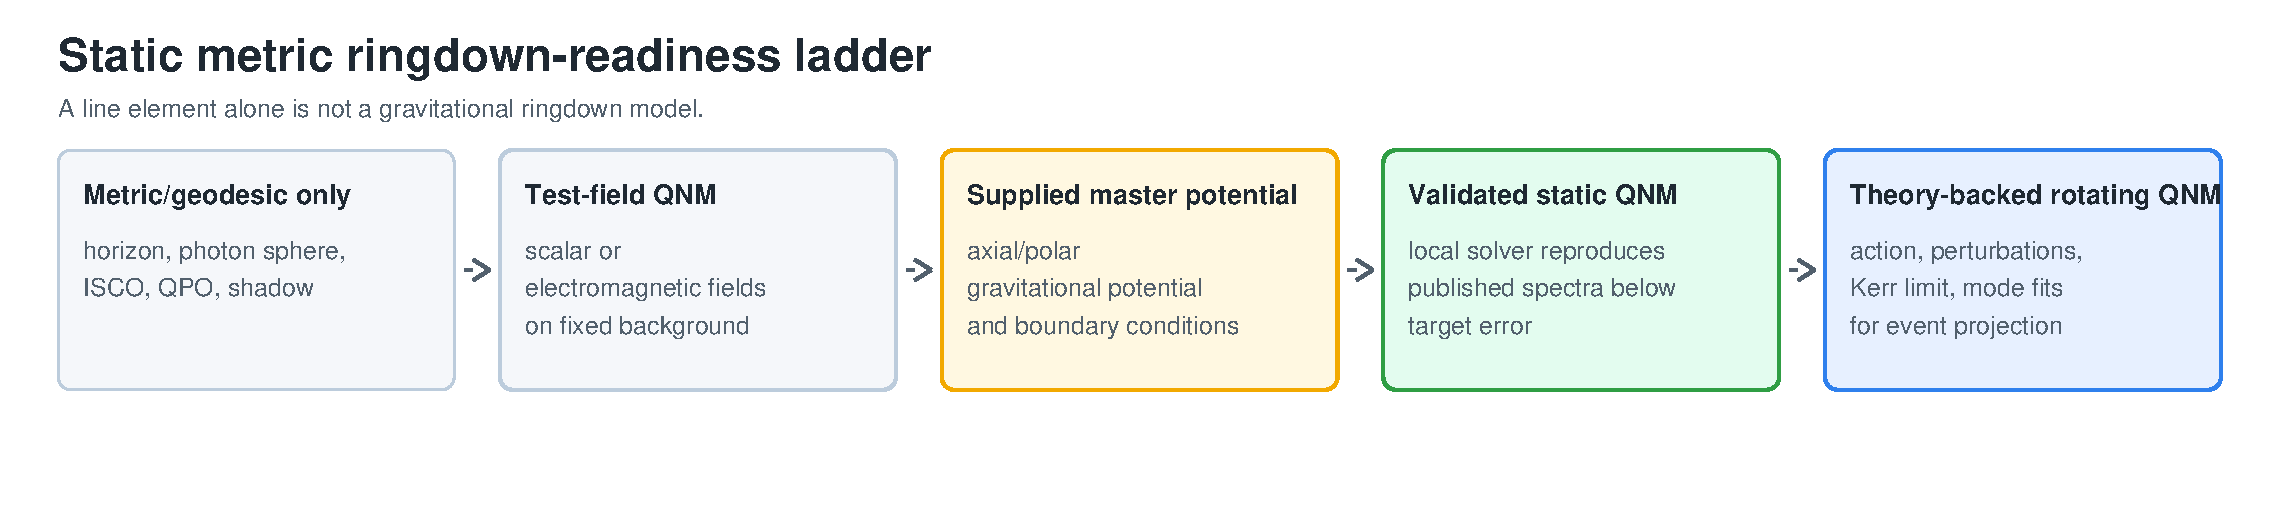
\includegraphics[width=0.9\textwidth]{figures/static_metric_readiness_ladder.pdf}%
}{%
\fbox{\begin{minipage}{0.86\textwidth}
\centering Static readiness ladder available as
\path{figures/static_metric_readiness_ladder.svg}.
Convert the SVG to PDF before final journal submission.
\end{minipage}}%
}
\caption{Ringdown-readiness ladder for metric models. A line element or geodesic observable is not sufficient for gravitational ringdown use without perturbation physics and a validated spectrum.}
\label{fig:readiness_ladder}
\end{figure*}

\subsection{Public GW250114 Inputs}

We use public GW250114 ringdown/spectroscopy products in two separate
projection branches. The RINGDOWN branch uses the posterior samples for

\begin{equation}
y_R=\{\log f_{220},\log f_{221},\delta f_{221}\}.
\end{equation}

The pyRing branch uses the 221 fractional deviation posterior

\begin{equation}
y_P=\{\log(1+\delta\omega_{221}),\log(1+\delta\tau_{221})\}.
\end{equation}

These two branches are treated as complementary public-product projections of
the same event. We compare them for consistency, but we do not combine them
statistically because they are not independent likelihoods.

\subsection{Kerr Baseline}

For each mode, the Kerr reference is represented by the complex dimensionless
frequency \cite{Ber-Car-Wil:2006:PRD:,Ste:2019:JOSS:}

\begin{equation}
M\omega_{\ell mn}(\chi)=M\omega_{R,\ell mn}(\chi)-i\,M/\tau_{\ell mn}(\chi).
\end{equation}

The physical frequency and damping time scale as

\begin{align}
f_{\ell mn}(M,\chi)&\propto \frac{\mathrm{Re}[M\omega_{\ell mn}(\chi)]}{M},\\
\tau_{\ell mn}(M,\chi)&\propto \frac{M}{|\mathrm{Im}[M\omega_{\ell mn}(\chi)]|}.
\end{align}

The RINGDOWN projection uses the Kerr baseline for the event remnant mass and
spin, and in this branch the linearized remnant-mass and remnant-spin
directions are profiled over. The pyRing variables are already fractional
deviations from the Kerr prediction, and therefore the baseline in the pyRing
branch is zero.

\subsection{Higher-Derivative QNM Fingerprints}

For each one-at-a-time EFT operator and polarization branch, the imported QNM
fingerprints give linear responses such as

\begin{align}
\frac{\partial \log f_{\ell mn}}{\partial \alpha},\qquad
\frac{\partial \log \tau_{\ell mn}}{\partial \alpha}.
\end{align}

The projected coupling $\alpha$ is therefore a local linear coordinate along a
published higher-derivative QNM fingerprint. We do not interpret it here as a
full nonlinear or multi-parameter exclusion of theory space.

\subsection{Gaussian Projection}

For a public posterior sample vector $y$, we calculate the sample mean $\mu$ and
covariance $C$. The local Gaussian chi-square is

\begin{equation}
\chi^2(p)=\left[\mu-y_{\rm model}(p)\right]^T C^{-1}\left[\mu-y_{\rm model}(p)\right].
\end{equation}

For the RINGDOWN branch, the linearized model residual is

\begin{equation}
r=\mu-y_{\rm Kerr}=N\theta+s\alpha,
\end{equation}

where $\theta=\{\delta\log M_f,\delta\chi_f\}$ contains nuisance directions and
$s$ is the EFT fingerprint column. The mass nuisance direction contributes
$\{-1,-1,0\}$ to $\{\log f_{220},\log f_{221},\delta f_{221}\}$. The spin nuisance direction
is evaluated numerically from the Kerr QNM sequence. For each EFT fingerprint
we solve the weighted least-squares problem and profile over the nuisance
directions.

For the pyRing branch, the model is

\begin{align}
y_P&=s\alpha,\\
s&=\left\{\frac{\partial\log f_{221}}{\partial\alpha},
\frac{\partial\log\tau_{221}}{\partial\alpha}\right\}.
\end{align}

No remnant-mass or remnant-spin nuisance profiling is used in this branch,
because the public variables are already given as fractional deviations
relative to the Kerr prediction.

For both branches, the reported Gaussian 90 percent interval is

\begin{equation}
\hat{\alpha}\pm 1.6448536269514722\,\sigma_{\alpha}.
\end{equation}

The result should be read as a public-data projection. It is not a Bayes
factor, not a model-selection statistic, and not a substitute for a full
strain-level likelihood with priors, waveform systematics, and nonlinear
parameter correlations.

The RINGDOWN construction profiles over the local mass and spin directions,
but this is still only a Gaussian projection of public posterior products. It
does not marginalize over the full nonlinear degeneracy between the remnant
parameters and the beyond-Kerr coupling, and it does not include alternative
ringdown start times, waveform systematics, calibration uncertainty, or a
penalty for the additional coupling. We keep these limitations explicit
because they define the boundary between the present public-data exercise and
a true event-level beyond-Kerr inference. In particular, the quoted intervals
should not be read as guaranteed conservative bounds. They can be narrower
than intervals from a full strain-level Bayesian analysis if nonlinear
mass-spin-coupling correlations or prior-volume effects are important.

\subsection{Static Supplied-Potential QNM Validation}

The static branch is separated from the GW250114 rotating-remnant projection.
For a supplied master potential, the local code evolves

\begin{equation}
\partial_t^2\Psi-\partial_x^2\Psi+V(r(x))\Psi=0,
\end{equation}

where $x$ is the tortoise coordinate. The extracted waveform is fitted with
Prony, linear-prediction, or matrix-pencil methods according to the mode
content. The validation target is not nature. It is the corresponding
published QNM table or the local Schwarzschild \texttt{qnm} reference.

This step tests reproducibility of a perturbative calculation. It does not
decide whether the corresponding metric is realized astrophysically. It also
does not make a static model directly comparable to the rotating GW250114
remnant.

\section{Results and Discussion}

\begin{figure*}[t]
\centering
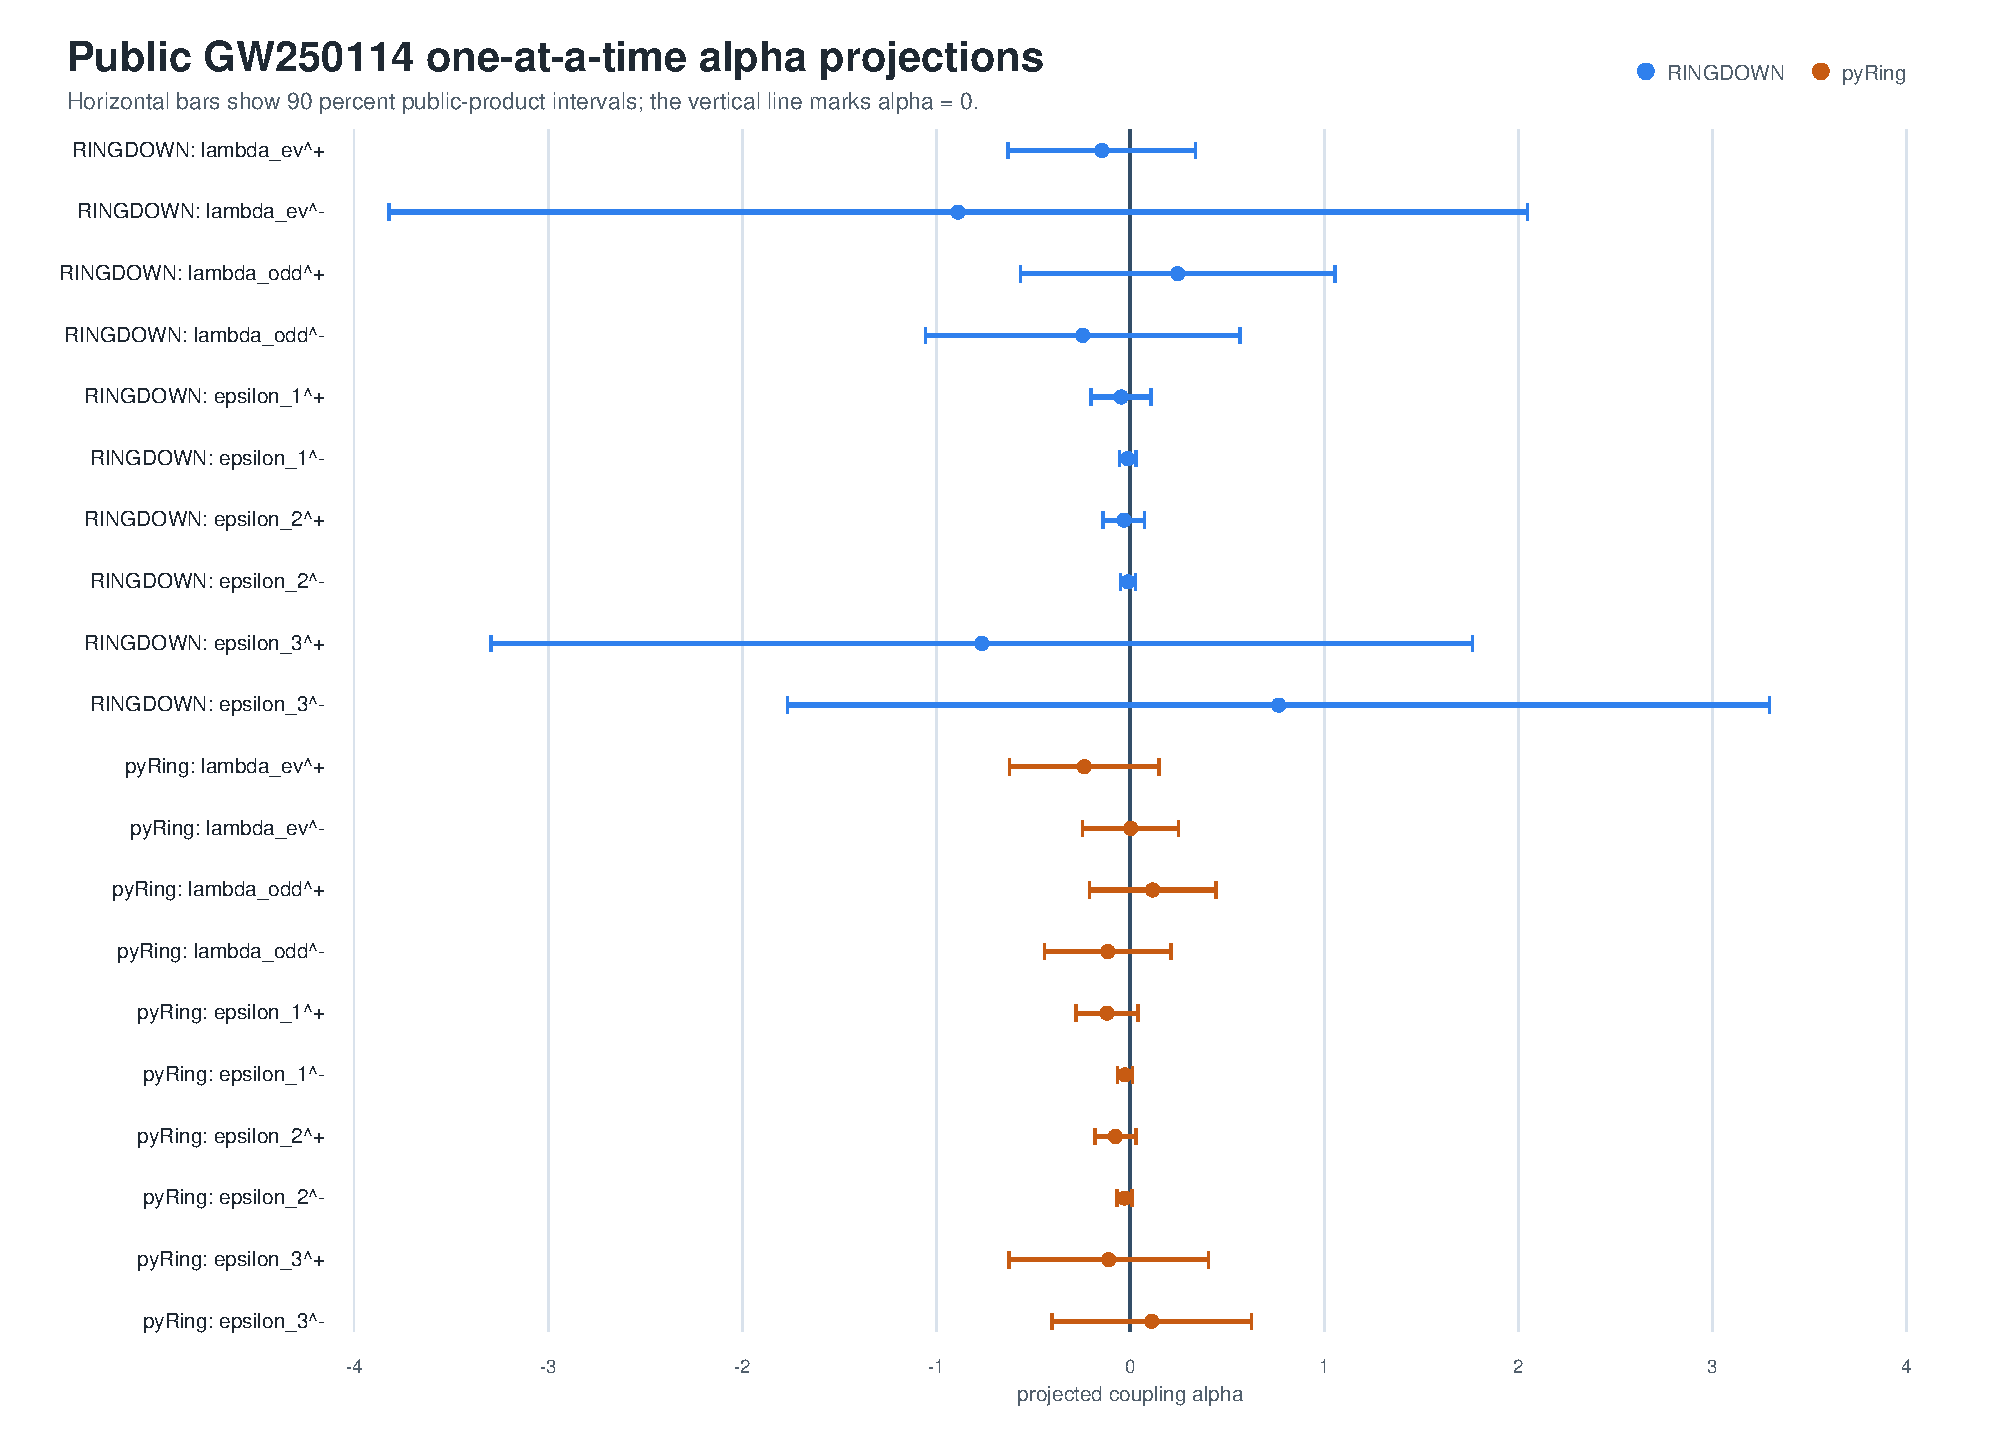
\includegraphics[width=0.95\textwidth]{figures/projection_alpha_interval_forest.pdf}
\caption{Forest plot of the one-at-a-time public GW250114 projections. Points show $\hat{\alpha}$ and bars show the 90 percent public-product intervals. The vertical line marks $\alpha=0$, which lies inside every interval in both the RINGDOWN and pyRing branches.}
\label{fig:public_projection_forest}
\end{figure*}

\begin{table*}
\caption{Public GW250114 higher-derivative QNM projections. The RINGDOWN and pyRing branches are reported separately and are compared but not statistically combined.}
\label{tab:public_projection_summary}
\begin{ruledtabular}
\begin{tabular}{lccccc}
Projection & Observables & Rows & Zero outside 90\% & Max statistic & Row \\
RINGDOWN & $\log f_{220}$, $\log f_{221}$, $\delta f_{221}$ & 10 & 0 & 0.497 & $\lambda_{\rm odd}^{+}$ \\
pyRing deviation & $\delta\omega_{221}$, $\delta\tau_{221}$ & 10 & 0 & 1.222 & $\epsilon_1^{+}$ \\
RINGDOWN vs. pyRing & operator comparison & 10 & 0 & 0.535 & $\epsilon_1^{+}$ \\
\end{tabular}
\end{ruledtabular}
\end{table*}

\begin{table*}
\caption{Per-operator public GW250114 projection values. The intervals are one-at-a-time 90 percent public-product intervals for the local linearized coupling $\alpha$; they are not Bayes factors and not multi-parameter EFT constraints.}
\label{tab:public_projection_detail}
\begin{ruledtabular}
\begin{tabular}{llccccc}
Branch & Operator & $\hat{\alpha}$ & $\sigma_{\alpha}$ & 90\% interval & $|\hat{\alpha}|/\sigma_{\alpha}$ & $\alpha=0$ inside \\
RINGDOWN & $\lambda_{\rm ev}^{+}$ & -0.146 & 0.294 & $[-0.630,\,0.337]$ & 0.497 & yes \\
RINGDOWN & $\lambda_{\rm ev}^{-}$ & -0.887 & 1.784 & $[-3.822,\,2.047]$ & 0.497 & yes \\
RINGDOWN & $\lambda_{\rm odd}^{+}$ & 0.245 & 0.492 & $[-0.565,\,1.055]$ & 0.497 & yes \\
RINGDOWN & $\lambda_{\rm odd}^{-}$ & -0.245 & 0.492 & $[-1.055,\,0.565]$ & 0.497 & yes \\
RINGDOWN & $\epsilon_1^{+}$ & -0.047 & 0.094 & $[-0.202,\,0.108]$ & 0.497 & yes \\
RINGDOWN & $\epsilon_1^{-}$ & -0.013 & 0.026 & $[-0.055,\,0.029]$ & 0.497 & yes \\
RINGDOWN & $\epsilon_2^{+}$ & -0.032 & 0.065 & $[-0.140,\,0.075]$ & 0.497 & yes \\
RINGDOWN & $\epsilon_2^{-}$ & -0.012 & 0.024 & $[-0.051,\,0.027]$ & 0.497 & yes \\
RINGDOWN & $\epsilon_3^{+}$ & -0.765 & 1.538 & $[-3.295,\,1.765]$ & 0.497 & yes \\
RINGDOWN & $\epsilon_3^{-}$ & 0.765 & 1.538 & $[-1.765,\,3.295]$ & 0.497 & yes \\
pyRing deviation & $\lambda_{\rm ev}^{+}$ & -0.237 & 0.234 & $[-0.622,\,0.148]$ & 1.013 & yes \\
pyRing deviation & $\lambda_{\rm ev}^{-}$ & 0.003 & 0.150 & $[-0.245,\,0.250]$ & 0.018 & yes \\
pyRing deviation & $\lambda_{\rm odd}^{+}$ & 0.116 & 0.198 & $[-0.211,\,0.442]$ & 0.583 & yes \\
pyRing deviation & $\lambda_{\rm odd}^{-}$ & -0.116 & 0.198 & $[-0.442,\,0.211]$ & 0.583 & yes \\
pyRing deviation & $\epsilon_1^{+}$ & -0.120 & 0.098 & $[-0.280,\,0.041]$ & 1.222 & yes \\
pyRing deviation & $\epsilon_1^{-}$ & -0.027 & 0.024 & $[-0.066,\,0.012]$ & 1.145 & yes \\
pyRing deviation & $\epsilon_2^{+}$ & -0.077 & 0.064 & $[-0.182,\,0.029]$ & 1.195 & yes \\
pyRing deviation & $\epsilon_2^{-}$ & -0.029 & 0.024 & $[-0.068,\,0.010]$ & 1.211 & yes \\
pyRing deviation & $\epsilon_3^{+}$ & -0.111 & 0.312 & $[-0.625,\,0.403]$ & 0.355 & yes \\
pyRing deviation & $\epsilon_3^{-}$ & 0.111 & 0.312 & $[-0.403,\,0.625]$ & 0.355 & yes \\
\end{tabular}
\end{ruledtabular}
\end{table*}

\subsection{Public GW250114 Projection}

The public RINGDOWN and pyRing branches give a consistent null result in the
linearized one-at-a-time higher-derivative projection. In the RINGDOWN branch,
all ten operator/polarization rows retain $\alpha=0$ inside the configured
90 percent Gaussian interval. The largest nominal displacement from zero is
$0.497\sigma$, in the $\lambda_{\rm odd}^{+}$ row.

The identical $0.497\sigma$ value appearing across the RINGDOWN rows is a
consequence of the local profiling geometry rather than an independent
coincidence in every operator. The RINGDOWN observable vector has three
components, and the projection profiles over two nuisance directions
associated with remnant mass and spin. The remaining projected residual is
therefore effectively one-dimensional. Different one-at-a-time fingerprint
columns mainly change the scale and sign of the inferred $\alpha$, while the
normalized distance of the public posterior mean from the profiled Kerr
surface remains the same at this order.

In the pyRing deviation branch, all ten rows again retain $\alpha=0$ inside
the 90 percent interval. The largest nominal displacement is $1.222\sigma$, in
the $\epsilon_1^{+}$ row.

The two branches should be interpreted as complementary projections of
overlapping public analyses, not as independent constraints. Their
operator-by-operator comparison gives a maximum normalized projection
difference of $0.535\sigma$ for the $\epsilon_1^{+}$ row. No row shows a
90 percent interval tension between the RINGDOWN and pyRing projections.

This is the sense in which the worked GW250114 example is a null result. It
does not prove that higher-derivative corrections are absent. It shows that,
within the public products and linearized one-at-a-time treatment used here,
there is no robust projected displacement from the Kerr value. The full
per-operator values of $\hat{\alpha}$, $\sigma_{\alpha}$, the 90 percent intervals,
and the branch-to-branch comparison are kept in the numerical tables so that
the summary statement can be checked without rerunning the code.

\subsection{Robustness Checks}

The pyRing lower-tail filter sweep supports the same null statement. Across
the stricter, public, looser, and positive-domain-only filter choices,
$\alpha=0$ remains inside every configured 90 percent interval. The largest
nominal filter-sweep displacement is $1.290\sigma$.

The empirical linearized posterior-sample projection gives the same qualitative
result without using only symmetric Gaussian intervals. In this check, no
empirical 90 percent interval excludes $\alpha=0$. The largest nominal
$|\mathrm{median}|/\sigma$ is $1.286$.

These checks support the stability of the public projection, but they are not
independent evidence and they do not replace a full Bayesian event-level
analysis. They address two limited failure modes of the Gaussian summary: the
choice of pyRing lower-tail filter and the use of a symmetric covariance
approximation. They do not test start-time dependence or waveform
model-dependence, because those choices are already built into the public
products used here.

\begin{table*}
\caption{Static supplied-potential QNM readiness summary. Validation errors quantify reproduction of reference spectra. The maximum physical shift is the largest sampled absolute relative change in either $\mathrm{Re}(M\omega)$ or $|\mathrm{Im}(M\omega)|$ from the Schwarzschild or zero-parameter baseline; it is not an observational exclusion interval.}
\label{tab:static_readiness_summary}
\begin{ruledtabular}
\begin{tabular}{lccccc}
Family & Modes & Rows & Max validation [\%] & Max physical shift [\%] & Largest sampled parameter \\
Bardeen NED & $\ell=2,n=0$ & 3 & 0.873 & 109.8 & $\alpha=0.7698$ \\
Braneworld tidal charge & $\ell=2,n=0$ & 5 & 0.454 & 21.214 & $q_{\rm tidal}=2$ \\
Hayward & $\ell=2,n=0$ & 6 & 0.718 & 16.596 & $\gamma=1.18$ \\
Hayward overtone & $\ell=2,n=1$ & 7 & 0.925 & 17.407 & $\gamma=1.18$ \\
Schwarzschild & $\ell=2,n=0$ & 4 & 0.432 & n/a & n/a \\
\end{tabular}
\end{ruledtabular}
\end{table*}

\subsection{Static QNM Benchmarks}

The static branch is included for one reason: it turns the readiness ladder
from a slogan into a reproducible test. We take examples that are not directly
usable for GW250114, but that do supply a gravitational master potential or a
published QNM reference, and ask whether the spectrum can be reproduced before
any phenomenological interpretation is attempted. The present validation
scorecard contains $25$ rows across Schwarzschild, braneworld tidal charge,
Bardeen NED, Hayward fundamental, and Hayward first-overtone examples. All
validation families pass the configured sub-percent criterion. The largest
validation discrepancy is $0.925\%$, for the Hayward first-overtone
matrix-pencil extraction. This number measures reproduction of a published
reference table, not agreement with observation.

In the static summary, \texttt{max physical shift} means the maximum sampled absolute
relative change, in percent, of either \texttt{Re(M omega)} or \texttt{Abs(Im(M omega))}
with respect to the stated Schwarzschild or zero-parameter baseline. It is not
a complex-norm posterior, not a detector-space residual, and not an
observational exclusion statistic.

After validation, the same static examples can be used to measure physical QNM
shifts relative to a Schwarzschild or zero-parameter baseline. These shifts are
larger than the numerical validation errors:

\begin{itemize}
\item Bardeen NED: maximum sampled shift $109.8\%$ at $\alpha=0.7698$;
\item braneworld tidal charge: maximum sampled shift $21.214\%$ at $q_{\rm tidal}=2$;
\item Hayward fundamental: maximum sampled shift $16.596\%$ at $\gamma=1.18$;
\item Hayward first overtone: maximum sampled shift $17.407\%$ at $\gamma=1.18$.
\end{itemize}

This shows that the static test is not only a numerical reproduction exercise.
The threshold-crossing table gives sparse-grid 1, 3, 5, and 10 percent
crossings. However, these are diagnostic interpolation results, not
observational exclusion intervals.

\subsection{Interpretation of the Static Branch}

The static benchmarks should be read as readiness tests, not as GW250114
constraints. They answer a limited but useful question: if a phenomenological
metric is supplied together with a gravitational master potential, can the QNM
spectrum be reproduced and used in a controlled stress test? For the examples
considered here the answer is yes at the static supplied-potential level.

This is different from saying that Bardeen, Hayward, tidal-charge, or other
static backgrounds are ruled out, preferred, or disfavoured by GW250114. Such a
claim would require a rotating solution, the correct perturbation system, mode
identification for the remnant spin, priors on the extra parameters, and an
observational likelihood at the same approximation level.

The usefulness of the static branch is therefore diagnostic. It identifies
where a model sits on the ladder from metric-only phenomenology to
ringdown-ready theory. A model used in QPO or shadow studies may be useful at
the geodesic level, but that does not make it a gravitational-ringdown model.
The readiness standard makes this distinction explicit.

\subsection{Limitations and Next Steps}

The public GW250114 projection is intentionally conservative. It is linearized,
tests one effective coupling at a time, and uses public posterior products
rather than a full strain-level beyond-Kerr likelihood. It does not compute
Bayes factors or information criteria, and it does not explore multi-parameter
EFT directions. It also does not scan ringdown start time, because the goal is
to project the released spectroscopy products rather than to redo the event
analysis. These are limitations of scope rather than hidden assumptions.

The most direct extension of the observational branch is a full event-level
likelihood using the strain data, detector noise model, ringdown start-time
treatment, and beyond-Kerr waveform response in one inference problem. A second
extension is to include multi-parameter EFT directions and nonlinear responses.

The most direct extension of the readiness branch is to add more
theory-complete or supplied-potential cases. Reissner-Nordstrom or
gravito-electromagnetic perturbations provide a clean charged benchmark.
Slow-rotation supplied-potential examples would be especially valuable,
because they would reduce the conceptual distance between static benchmarks
and high-spin merger remnants without requiring a full generic rotating
solution. Dynamical Chern-Simons or other theory-backed rotating calculations
\cite{Chu-Lam-Yun:2025:PRD:,Li-Wag-Che:2025:ARXIV:,Pie-Gua:2022:PRD:} could be
more directly connected to high-spin remnant spectroscopy if the required mode
set is available. The criterion should remain the same: the model must provide
enough perturbation information to compute or reproduce gravitational QNM
spectra.

The main value of the present work is therefore not a claim of new physics. It
is a reproducible public-data example plus a ringdown-readiness standard. The
first part keeps observational statements controlled, while the second part
keeps theoretical phenomenology controlled. Together they define a practical
standard for future high-SNR ringdown events and for the alternative metrics
proposed to interpret them.

\section*{Data and Code Availability}

All scripts, configuration files, intermediate tables, validation summaries,
and manuscript-supporting outputs are included in the accompanying repository.
The public GW250114 inputs are drawn from the GWOSC/Zenodo event release. The
higher-derivative QNM fingerprints are imported from the public
BeyondKerrQNM/Cano et al. fit data. Static benchmark inputs are derived from
the cited published master potentials and QNM tables. The working repository
placeholder is \url{https://github.com/jvrba/gw250114-ringdown-readiness}; this
placeholder should be replaced by the final public archive before journal
submission.

\clearpage
\bibliographystyle{apsrev4-2}
\bibliography{references}

\end{document}
